\section{Diffraction of Light Through a Single Slit}

\makelabheader %(Space for student name, etc., defined in master.tex)

\bigskip
\textbf{Apparatus}

\begin{itemize}[nosep]
\item Basic optics diode laser
\item Optical bench with rotary motion sensor
\item Phototransistor for measuring light intensity (mounted on rotary motion sensor)
\item ``Single Slit Set'' slit accessory
\item ``Multiple Slit Set'' slit accessory
\item Small plastic ruler
%\item Glass plate with sets of narrow slits
\item Pasco 550 Interface
\item \textit{Capstone} software (\filename{Interference.cap} experiment file)
\item \textit{Mathematica} software (\filename{diffraction.nb} notebook file)
\end{itemize}

\bigskip
\textbf{Activity 1: Making Predictions and Taking Data}

(a) In the previous lab, you saw that laser light emitted from two slits can interfere with each other.  If you shine laser light through a single slit, do you predict that you will see any evidence of constructive or destructive interference?  Why or why not?
\answerspace{0.8in}


Well, let's try it!  The setup for this experiment is exactly the same as that for Lab \ref{interference_lab},  but instead of a double slit, you will use the ``Single Slit Set'' slit accessory.  Place it on the optical bench about 70 cm away from the detector, and select the slit with a width of $a = 0.16$~mm.   Set the gain switch to 100 and use the aperture marked ``3''.   Open the file \filename{Interference.cap} and use the computer to take data on the intensity as a function of position by moving the detector slowly across the series of bright spots.  

Your goal is to get as large a signal as you can without having the intensity pinned at its maximum value.  (If the peaks on your graph appear perfectly flat on top, that's probably what's happening.) You may need to adjust either the gain of your detector or the size of its aperture.

(b) In the space below, draw a good, careful graph showing the ``diffraction pattern'' you see.  
Be sure to label your axes!
\answerspace{1.5in}

\pagebreak[2]
\textbf{Activity 2: Understanding What's Going On}

The complex pattern of maxima and minima that you see doesn't look anything like a simple shadow of the single slit.  In fact, it looks a little bit like the kind of interference pattern you get from shining light through two narrow slits.  But what's with that?  How can you have interference from only one slit?

Although there is only one slit, light still comes from many different places \textit{within} the slit: the left side, the right side, or anywhere in between.  In fact, we could draw an \textit{infinite} number of rays coming from all locations, and going in all directions, as in the drawing (a) below.  But as before, we'll consider rays traveling only in one particular direction $\theta$ at a time.  The drawing (b) below shows eight evenly spaced rays, numbered 1 through 8.  The pink area behind them reminds us that there are really an infinite number of rays in that direction.

\answerspace{0.2in}
\begin{center}
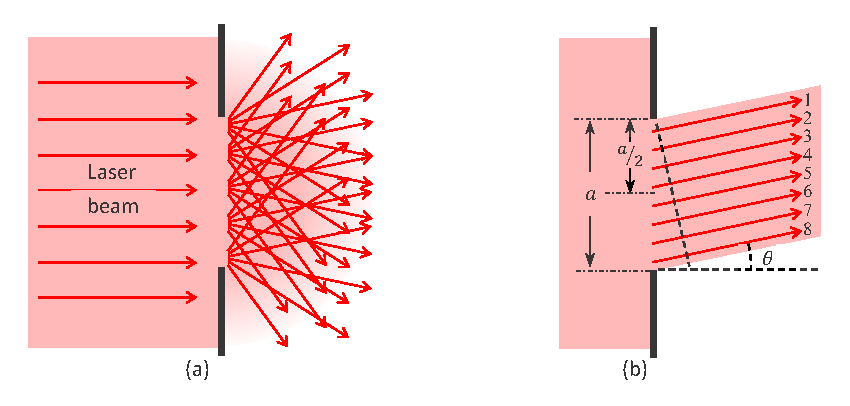
\includegraphics{diffraction_of_light/one_slit_rays_color.eps}
\end{center}
\index{color_page}
\answerspace{0.2in}

(a) For a particular angle $\theta$ where the path difference between rays 1 and 5 is given by $\Delta r_{15}=\frac{1}{2}\lambda$, will rays 1 and 5 interfere \textit{CON-structrively} or \textit{DE-structively}?
\answerspace{0.4in}

(b) For an angle $\theta$ where $\Delta r_{15}=\frac{1}{2}\lambda$, what is $\Delta r_{26}$?  What about $\Delta r_{37}$? And $\Delta r_{48}$?
\answerspace{0.5in}

(c) At the particular angle $\theta$ where $\Delta r_{15}=\frac{1}{2}\lambda$, will the intensity at the screen be a maximum, zero, or something in between?
\answerspace{0.4in}

(d) What is $\Delta r_{15}$ in terms of $a$ and $\theta$?
\answerspace{0.4in}

The upshot of this is that for a single slit, you should have an intensity minimum, with complete destructive interference, at the particular angle $\theta$ where $\frac{a}{2} \sin \theta = \frac{1}{2}\lambda$.  In the next activity, you'll see whether there are other angles for which that's also true.

\pagebreak[3]
To help you visualize what's happening, open the file \filename{diffraction.nb} in the \filename{\coursefolder} folder; 
it will open in \textit{Mathematica}.  Hit \button{Control-A} to select all the text, and \button{Shift-Enter} 
to execute all of the selected text.  Scroll down until you see the graphics, and make the window full screen so the graphics all fits side by side.  You should see something like the screen shot below.

{\centering 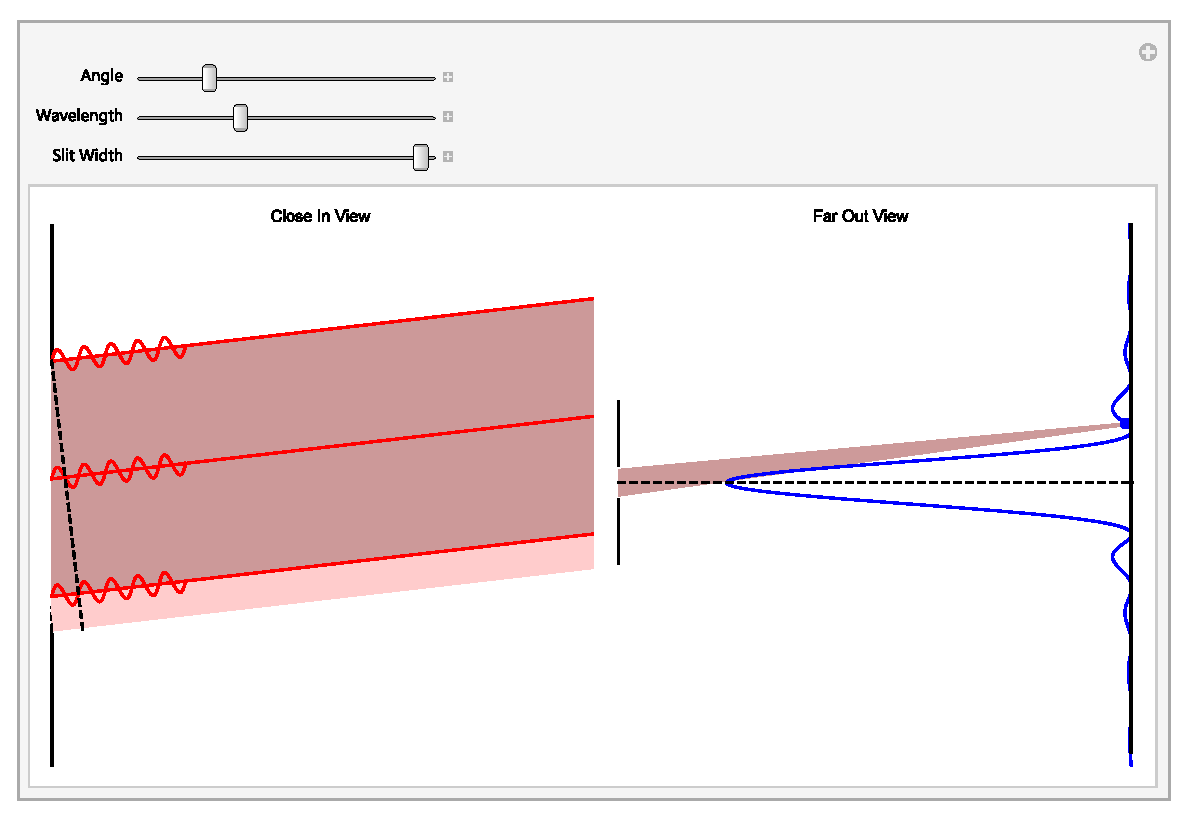
\includegraphics[height=4.1in]{diffraction_of_light/one_slit_screengrab.eps} \par}
\index{color_page}

The ``Close In View'' shows a wide band of pink (and slightly grayed-out pink) that represents the infinite number of rays at the given angle.  In the screenshot above, there are also three specific rays that are drawn in red: one at the very top of the band, and two more with path lengths $\Delta r$ that differ from the topmost ray by $\frac{1}{2} \lambda$ and $\lambda$.  As you adjust the angle slider, you'll see that the number of rays drawn changes, but that the rays drawn always have half-integer path differences from each other. 

(e) In the screenshot above, the topmost ray drawn exactly cancels the middle ray, because their path difference is $\Delta r = \frac{1}{2} \lambda$, so they interfere \textit{destructively}.  Draw an additional ray in the picture exactly between those two rays.  Is there another ray somewhere in the band that would exactly cancel the one you drew?  If yes, draw that ray as well.  If no, then explain why below.
\answerspace{0.5in}

(f) Is every possible ray between the top and middle rays drawn in the picture exactly canceled by another ray somewhere else in the band?
\answerspace{0.4in}

(g) Why is most of the band in the picture above colored as a grayed-out pink instead of a brighter pink?
\answerspace{0.4in}

(h) Label in the picture above the part of the band that actually contributes to a non-zero intensity at the detector at the angle pictured.

\pagebreak[3]
\textbf{Activity 3: Finding All Intensity Minima}


\vspace{-0.2in}
\begin{center}
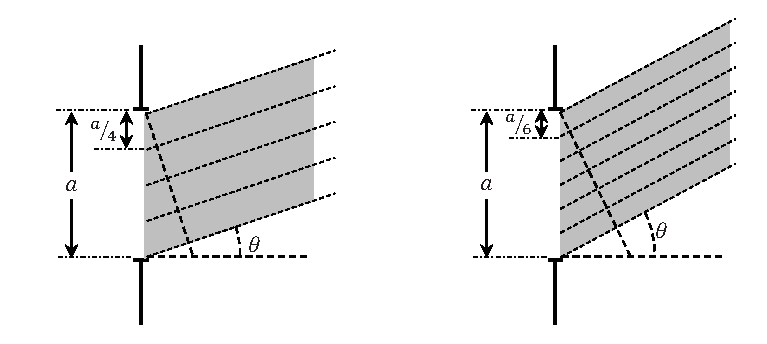
\includegraphics[width=0.7\textwidth]{diffraction_of_light/fourths_and_sixths.eps}
\end{center}
\vspace{-0.2in}

(a) Looking at the left diagram above, write a condition for when the top-most ray will interfere destructively with the ray $\frac{a}{4}$ from the top.  Your equation should be in terms of $a$, $\sin \theta$, and $\lambda$.  
\answerspace{0.4in}

(b) Considering \textit{all} rays at that angle $\theta$, will your condition lead to an intensity minimum with complete destructive interference?  Why or why not?
\answerspace{0.4in}

(c) Looking at the right diagram above, write a condition for when the top-most ray will interfere destructively with the ray $\frac{a}{6}$ from the top.  (Again, in terms of $a$, $\sin \theta$, and $\lambda$.)  Will this condition also lead to an overall intensity minimum?
\answerspace{0.4in}

(d) It looks like you could keep dividing the slit into any even number of sections and get the same result.  Write a generalized version of your condition for an intensity minimum in terms of an arbitrary integer $m$.  (You can cancel out a two to simplify your result.)

\answerspace{0.1in}
\hspace{0.8in}\textit{For a single slit of width \textit{a}, intensity \textit{minima} occur where: }
\answerspace{0.1in}

(e) Is your expression true for $m=0$?
\answerspace{0.4in}

(f) The diffraction pattern for a single slit is shown below.  Label all of the minima with the corresponding value $m=1$, $m=2$, etc.  
\label{fraunhofer_graph}

%\vspace{-0.2in}
%\begin{center}
%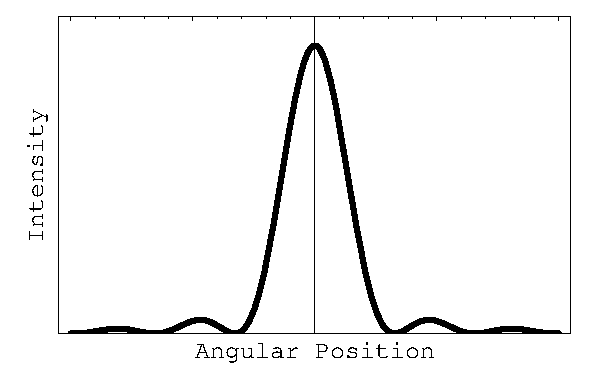
\includegraphics[width=0.4\textwidth]{diffraction_of_light/diffraction_of_light_fig_3.eps}
%\end{center}
%\vspace{-0.2in}
\begin{lab_axis}*[lab_noticks_4quads,
	width=4.5in,height=1.5in,
	xmin=-12,xmax=12,
	ymin=0,ymax=1.2,
	ylabel=Intensity,
	xlabel=Angular Position,
	xtick={.1}, % it won't let me put the tick exactly at zero.
	tick style={major tick length=0pt},
	axis y line*= {middle, y axis line style={->}}, %This effectively makes the graph only quadrants I and II
	xticklabel={0$^\circ$},
]
\addplot {(sin(deg(x))/x)^2};
\end{lab_axis}

\pagebreak[3]

(g) Calculate the angular separation $\theta$ between the central maximum and any numbered minimum you choose in your data, using measurements of $L$ and $\Delta x$ for that minimum.  Use your value for $\theta$ and your expression in part (d) to calculate the width $a$ of the slit.  (The wavelength of the light from your laser is 650 nm.  To get $\theta$, you'll need to measure the distance from the slit to the detector and do some calculations.)    Does your value of $a$ agree with what is written on the slit?
\answerspace{1.0in}


\textbf{Activity 4: Why Are Some Intensity Maxima Brighter?}

The diagram below shows what happens when all of the rays in a single direction don't neatly divide into an even number of groups that cancel each other out.

{\centering 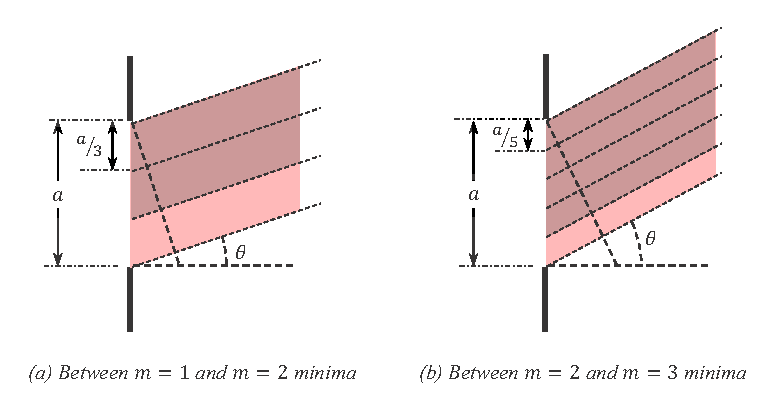
\includegraphics{diffraction_of_light/diffraction_maxima_color.eps} \par}
\index{color_page}

The diagram on the left shows rays at an angle $\theta$ where $\frac{a}{3} \sin \theta = \frac{\lambda}{2}$.  In the upper shaded area of the diagram, each ray can be \textit{paired up} with another one exactly $180^{\circ}$ out of phase, so that all of the rays inside that shaded area cancel each other out.  The intensity at the screen or the detector  comes from the unpaired rays that aren't shaded out.

(a) If $\theta$ were \textit{just a little} smaller than what's shown in the left diagram, would the resulting intensity \textit{increase}, \textit{decrease}, or \textit{stay the same}? (If you're not sure, you can always try it out on the simulation.)
\answerspace{0.4in}

(b) If $theta$ were \textit{just a little} bigger than what's shown in the diagram, would the resulting intensity \textit{increase}, \textit{decrease}, or \textit{stay the same}?  
\answerspace{0.4in}

(c) The particular $\theta$ shown in the diagram on the left is a maximum in the diffraction pattern.  Is the intensity of that maximum \textit{greater than}, \textit{less than}, or \textit{equal to} the intensity of the maximum at $\theta = 0$?  Why?
\answerspace{0.4in}

\pagebreak[2]
(d) Is the intensity of the maximum shown in the diagram on the right \textit{greater than}, \textit{less than}, or \textit{equal to} the intensity of the maximum shown on the left?  Why?  
\answerspace{0.4in}

(e) Are your answers for the last two questions consistent with the data you took for the single slit diffraction pattern, as well as the graph on page \pageref{fraunhofer_graph}?
\answerspace{0.4in}


\pagebreak[2]
\medskip
\textbf{Activity 5: Two-Slit Interference Revisited}

(a) Replace the single slit with the ``Multiple Slit Set'' slit accessory, and select the pair of two slits with separation $d=0.125$ mm and width $a=0.04$ mm, labeled with the number ``2''.  Get some good clean data on the intensity $I$ \textit{vs.}~position.

(b) As we described it in Lab \ref{interference_lab}, the two-slit interference pattern you see occurs because of the interference between rays coming from the exact center of each slit.  But if that were all that were going on,
the intensity function $I_{\rm 2slit}(\theta)$ would be a simple oscillating function with all maxima at exactly the same intensity:
\begin{displaymath} 
I_{\rm 2slit}(\theta) = I_{\rm{max}} \cos^2 \left (\frac {\pi d} {\lambda} \sin \theta \right) 
\end{displaymath}
(It's a little hard to parse, but for any $\theta$ where $d \sin \theta = m \lambda$, the part inside the parentheses gives a multiple of $\pi$ so that the value of the function is just $I_max$.)  Is that actually what you see?  If not, then how is your data different from the function above?
\answerspace{0.6in}

In fact, you probably see something more like the figure below, with some large maxima near the center, and several other much smaller maxima on either side.  (If you didn't see this, try increasing your signal strength, or consult your instructor.)

%\vspace{-0.1in}
%\begin{center}
%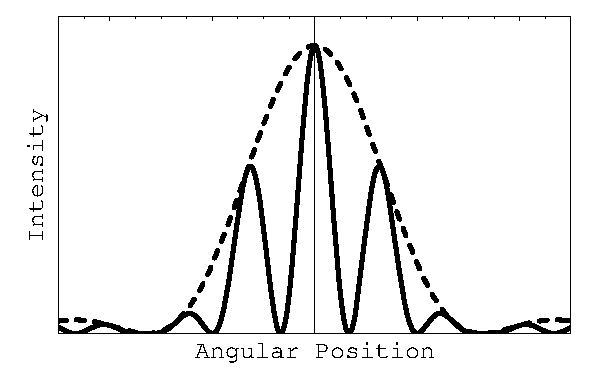
\includegraphics[width=0.4\textwidth]{diffraction_of_light/diffraction_of_light_fig_4.eps}
%\end{center}
%\vspace{-0.1in}
\begin{lab_axis}*[lab_noticks_4quads,
	width=4.5in,height=1.5in,
	xmin=-7,xmax=7,
	ymin=0,ymax=1.2,
	ylabel=Intensity,
	xlabel=Angular Position,
	xtick={.1}, % it won't let me put the tick exactly at zero.
	tick style={major tick length=0pt},
	axis y line*= {middle, y axis line style={->}}, %This effectively makes the graph only quadrants I and II
	xticklabel={0$^\circ$},
	samples = 800,
]
\addplot +[dashed, very thick] {(sin(deg(x))/x)^2};
\addplot {(cos(deg(4*x)))^2*(sin(deg(x))/x)^2};
\end{lab_axis}



The reason for the more complicated pattern is that in addition to the interference between rays from the two different slits, each individual slit has a nonzero width $a$, so there's also interference among different rays coming from the \textit{same} slit.  Essentially, the peaks from CON-structive interference \textit{between} the two slits get reduced due to DE-structive interference \textit{within} each slit.

\pagebreak[2]
Although the derivation goes beyond the scope of this course, the intensity function $I_{\rm{diff}}(\theta)$ for the diffraction of a single slit can actually be written in closed form as
\begin{displaymath} 
I_{\rm{diff}}(\theta) = I_{\rm{max}} \left( \frac {\sin \left(\frac {\pi a} {\lambda} \sin \theta \right)} {\frac {\pi a} {\lambda} \sin \theta} \right)^2 
\end{displaymath}
where $a$ is the width of the single slit, \( \theta  \) is the angular
position of the phototransistor relative to the incident beam, and $I_{\rm{max}}$
is the maximum intensity at the center of the diffraction pattern.  This is the function that's graphed on page \pageref{fraunhofer_graph}.




The complicated pattern you see is basically the simple oscillating function for two slit interference $I_{\rm 2slit}(\theta)$ multiplied by the intensity $I_{\rm{diff}}(\theta)$ at that angle for a single slit: 
\begin{displaymath} 
I_{\rm{total}} = I_{\rm{max}} \cos^2 \left (\frac {\pi d} {\lambda} \sin \theta \right) \left(\frac {\sin \left (\frac {\pi a} {\lambda} \sin \theta \right )} {\frac {\pi a} {\lambda} \sin \theta} \right)^2 \end{displaymath}

(c) Looking at your data, identify the position at which the interference maxima  are reduced to zero by the $m=1$ minimum of the single slit diffraction pattern.  Use that angle to calculate the apparent width $a$ of the slits.  Is it consistent with what is written on the slits?
\answerspace{0.5in}
